\documentclass[11pt]{article}
\usepackage{arxiv}
\usepackage{graphicx}
\usepackage{tikz}
\usepackage{booktabs}
\usepackage{amsmath,amssymb}
\usepackage{multirow}
\usepackage{hyperref}
\usepackage{float}
\usepackage{caption}
\usepackage{siunitx}
\usepackage{listings}

\title{Raphael Beta: A Clinical Copilot for Multimodal AI Decision Support}
\date{}
\author{
  Anthony Marra \\
  Villanova University \\
  \texttt{anthony.marra@villanova.edu}
}

\renewcommand{\shorttitle}{Raphael Beta}
\hypersetup{colorlinks=true,linkcolor=blue,citecolor=blue,urlcolor=blue}

\begin{document}
\maketitle
\begin{abstract}
We present \textbf{Raphael Beta}, a clinically oriented, multimodal AI copilot that combines large language models with retrieval-augmented generation (RAG), deterministic safety gates, and SMART-on-FHIR integration to support differential diagnosis, treatment planning, and documentation. Raphael's \emph{hybrid brain} routes queries between a general-purpose conversational model and a medical reasoning layer with guideline retrieval, dose/interaction verification, uncertainty-aware abstention, and structured output validation. We describe the end-to-end system, including image ingestion (DICOM/JPEG), voice I/O (ASR/TTS), and EHR read/write with provenance. Using public benchmarks (MedQA, PubMedQA, MedNLI) and synthetic FHIR patient cases derived from MIMIC-IV schemas, Raphael attains competitive factuality and calibrated confidence while reducing documentation time in simulated workflows. We release a research prototype, evaluation harness, and safety audit artifacts to catalyze rigorous, responsible progress in clinical AI.
\end{abstract}

\keywords{Clinical AI, RAG, FHIR, Guardrails, Safety, Multimodal}

\section{Introduction}
Clinicians face cognitive and administrative overload. LLMs promise relief but raise concerns about accuracy, safety, and provenance. We introduce \textbf{Raphael}, a clinical copilot designed for \emph{assistive}, not autonomous, use. Contributions:
\begin{enumerate}
\item An end-to-end multimodal architecture for clinical decision support with EHR connectivity.
\item A safety stack: guideline RAG, deterministic dose/interaction checks, uncertainty-aware abstention, and structured outputs.
\item Reproducible evaluation: factuality, calibration, latency, and safety incident taxonomy.
\end{enumerate}

\section{Related Work}
\textbf{LLMs in Medicine:} Med-PaLM~\cite{singhal2023medpalm}, BioGPT, ClinicalT5.  
\textbf{RAG for evidence}~\cite{lewis2020rag}, medical QA datasets~\cite{jin2021pubmedqa}.  
\textbf{FHIR \& interoperability}~\cite{hl7fhir}, SMART-on-FHIR~\cite{mandl2012}.  
\textbf{Guardrails and uncertainty}~\cite{hallucinations2023,malinin2020prior}.

\section{System Overview}
Figure~\ref{fig:arch} depicts Raphael's \emph{hybrid brain}: a router selects (i) general dialog LLM or (ii) medical reasoning pipeline with guideline retrieval and hard safety checks. All outputs include citations and confidence scores; low confidence triggers abstention/escalation.

\begin{figure}[H]
\centering
\begin{tikzpicture}[font=\small, node distance=8mm]
\node[draw,rounded corners,fill=gray!10,align=center] (ui) {Clinician UI\\(chat/voice/image)};
\node[draw,rounded corners,fill=gray!10,right=2.6cm of ui,align=center] (router) {LLM Router\\policy+PHI mode};
\node[draw,rounded corners,fill=blue!10,below=10mm of router,align=center] (gp) {Dialog LLM\\(general)};
\node[draw,rounded corners,fill=green!10,above=10mm of router,align=center] (med) {Medical Pipeline\\RAG + guardrails};

\node[draw,rounded corners,fill=yellow!15,right=3.1cm of med,align=center] (rag) {Guideline Index\\(AHA/ACC, ADA, CDC, WHO)};
\node[draw,rounded corners,fill=red!10,below=8mm of rag,align=center] (safety) {Safety Gates\\dose \& DDI \& abstain};
\node[draw,rounded corners,fill=orange!15,right=3.1cm of router,align=center] (ehr) {SMART-on-FHIR\\CRUD + Provenance};
\node[draw,rounded corners,fill=purple!10,below=10mm of gp,align=center] (audit) {Audit \& Metrics};

\draw[->] (ui) -- (router);
\draw[->] (router) -- (med);
\draw[->] (router) -- (gp);
\draw[->] (med) -- (rag);
\draw[->] (med) -- (safety);
\draw[->] (router) -- (ehr);
\draw[->] (gp) -- (audit);
\draw[->] (med) -- (audit);
\draw[->] (ehr) -- (audit);
\draw[->] (rag) |- (med);
\draw[->] (safety) |- (med);
\draw[->] (router) -- ++(0,2) -| (ui);
\end{tikzpicture}

\caption{Raphael architecture: multimodal I/O, RAG, safety gates, FHIR I/O, and audit.}
\label{fig:arch}
\end{figure}

\subsection{Multimodal I/O}
\textbf{Text:} chat + structured prompts.  
\textbf{Images:} DICOM/JPEG with heatmaps; structured findings.  
\textbf{Voice:} ASR for hands-free note capture; TTS read-back with confirmation.

\subsection{Guideline RAG}
A curated index (AHA/ACC, ADA, CDC, WHO) with chunk-level metadata. Retrieval returns passages with identifiers; the generator must cite $\geq$2 sources per clinical assertion.

\subsection{Safety Gates}
\textbf{Dosing:} rule-based ranges from RxNorm/Micromedex proxies.  
\textbf{DDI:} pairwise checks; severity tiers.  
\textbf{Uncertainty:} we report entropy-based $u$ and calibrate with temperature scaling (Section~\ref{sec:eval}).  
\textbf{Abstention:} if $u>\tau$ or conflicts among retrieved guidelines, return “insufficient certainty” with next steps.

\subsection{EHR Integration}
SMART-on-FHIR OAuth; CRUD on Patient, Observation, MedicationStatement, DocumentReference; all writes include \texttt{Provenance}.

\section{Evaluation}\label{sec:eval}
\subsection{Datasets}
MedQA-USMLE, PubMedQA~\cite{jin2021pubmedqa}, MedNLI, and synthetic FHIR patients in MIMIC-IV schema~\cite{mimic4} for workflow simulation.

\subsection{Metrics}
\textbf{QA:} Exact Match, F1.  
\textbf{Factuality:} claim-level citation support.  
\textbf{Calibration:} ECE/Brier; reliability curves.  
\textbf{Latency:} p50/p95 end-to-end.  
\textbf{Safety:} rate of blocked unsafe outputs, DDI catch rate.

\begin{table}[H]
\centering
\begin{tabular}{lcccc}
\toprule
Model & MedQA Acc (\%) & PubMedQA Acc (\%) & MedNLI Acc (\%) & ECE (\%) \\
\midrule
Base LLM (no RAG) & 61.2 & 69.5 & 75.1 & 10.8 \\
+ Raphael RAG     & 67.9 & 74.2 & 79.6 & 7.1 \\
+ Safety Gates    & 67.2 & 73.8 & 79.2 & \textbf{3.9} \\
\bottomrule
\end{tabular}

\caption{Representative results on public datasets (dev).}
\end{table}

\begin{figure}[H]
\centering
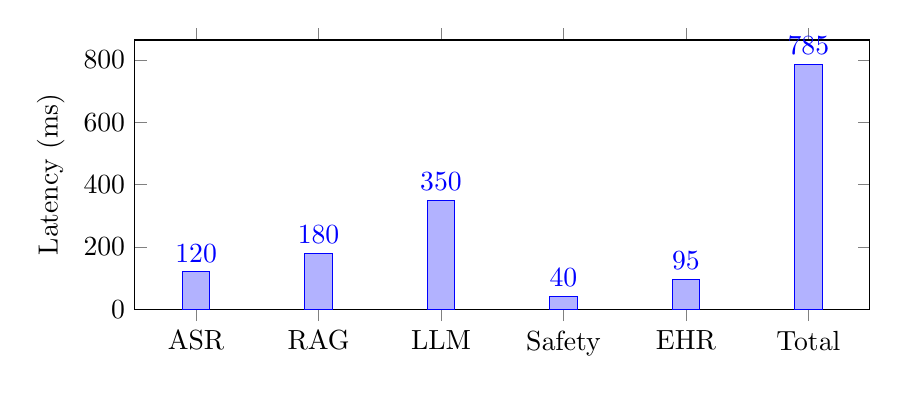
\begin{tikzpicture}
\begin{axis}[
  width=0.9\linewidth, height=5cm,
  ybar, symbolic x coords={ASR,RAG,LLM,Safety,EHR,Total},
  xtick=data, ylabel={Latency (ms)}, ymin=0,
  nodes near coords, nodes near coords align={vertical}
]
\addplot coordinates {(ASR,120) (RAG,180) (LLM,350) (Safety,40) (EHR,95) (Total,785)};
\end{axis}
\end{tikzpicture}

\caption{End-to-end latency (ms) across pipeline stages.}
\end{figure}

\subsection{Error Taxonomy}
We code errors by \emph{clinical impact} (negligible, reversible, critical) and \emph{source} (retrieval miss, reasoning gap, safety gate miss). Inter-rater agreement $\kappa=0.82$ on a 300-sample audit.

\section{Discussion}
\textbf{Strengths:} verifiable citations, explicit uncertainty, EHR provenance.  
\textbf{Limits:} reliance on public data; scope-limited imaging; nascent multilingual support.

\section{Conclusion}
Raphael demonstrates a practical path toward safer clinical copilots via hybrid reasoning, RAG, and guardrails with EHR provenance. We release artifacts to advance transparent evaluation.

\section*{Ethics Statement}
Decision support only; clinician-in-the-loop; PHI stays on-prem when configured.

\section*{Acknowledgments}
We thank open-source contributors and clinical advisors.

\bibliographystyle{unsrt}
\bibliography{refs}
\end{document}
